\section*{2. Расчет по постоянному току (DC анализ) нелинейной модели}

Для проведения анализа по постоянному току используется схема (файл примера \verb|LNA_DC_IV_start|), в которую интегрирована нелинейная SPICE-модель транзистора NE68133 (файл \verb|NE68133Package.lib|). Схема запитана от двух независимых источников напряжения постоянного тока: смещения на базе $V_B$ и напряжения на коллекторе $V_C$. Развязка по постоянному току обеспечивается дросселями индуктивностью 10 нГн и разделительными конденсаторами 10 пФ. Для контроля коллекторного тока $I_c$ в цепь последовательно включен виртуальный амперметр.

\begin{figure}[H]
	\centering
	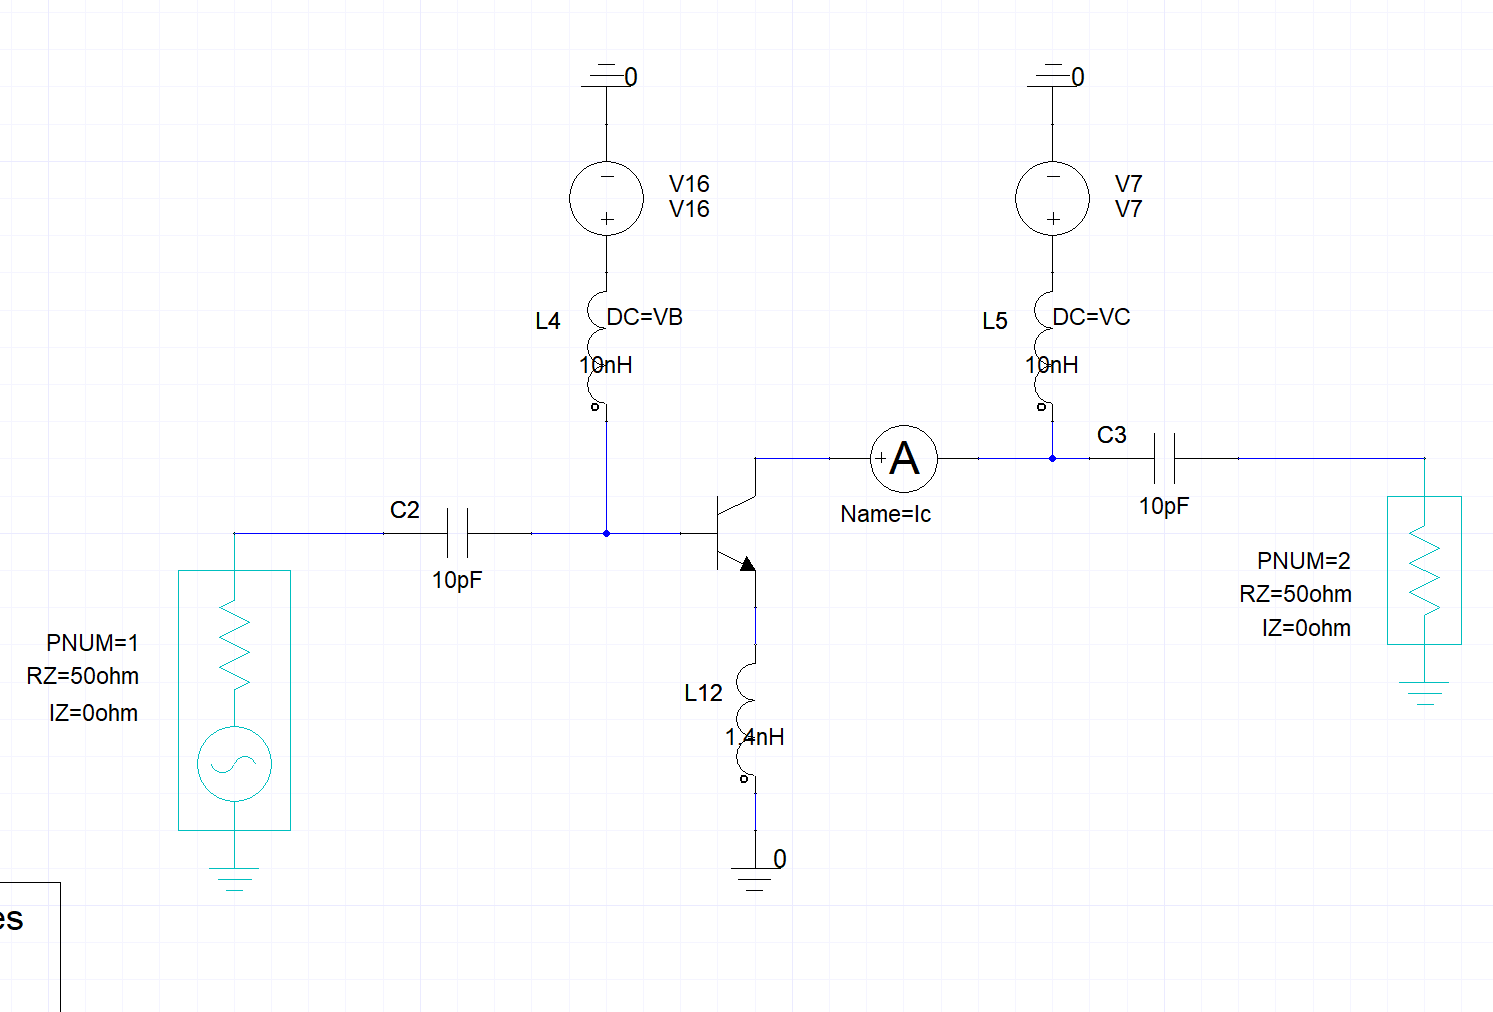
\includegraphics[width=0.8\textwidth]{9.PNG}
	\caption{Схема для DC анализа с нелинейной моделью транзистора.}
	\label{fig:dc_schema}
\end{figure}

Расчет семейства выходных вольтамперных характеристик (ВАХ) транзистора выполняется с помощью инструмента \verb|DC Analysis| (\verb|Analysis -> Add Nexxim Solution Setup -> DC Analysis|). 

\begin{figure}[H]
	\centering
	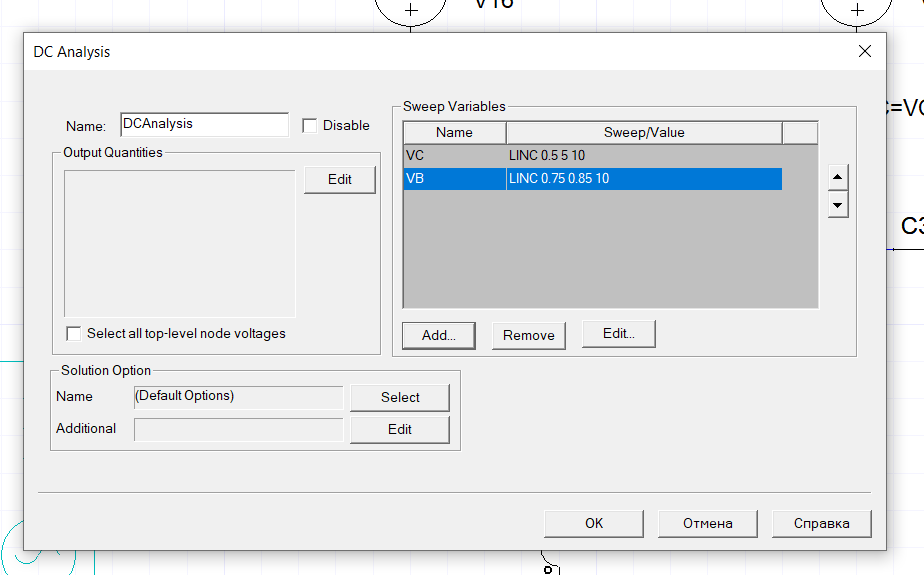
\includegraphics[width=0.7\textwidth]{8.PNG}
	\caption{Окно настройки параметров развертки (Sweep Variables) для DC анализа.}
	\label{fig:dc_setup_1}
\end{figure}

Для получения набора кривых задаются параметры развертки напряжений (Sweep Variables). Напряжение на базе $V_B$ изменяется в рабочем диапазоне от 0.75 В до 0.85 В с 10 шагами (LINC 0.75 0.85 10). Напряжение на коллекторе $V_C$ варьируется от 0.5 В до 5 В, также с 10 шагами (LINC 0.5 5 10).

\begin{figure}[H]
	\centering
	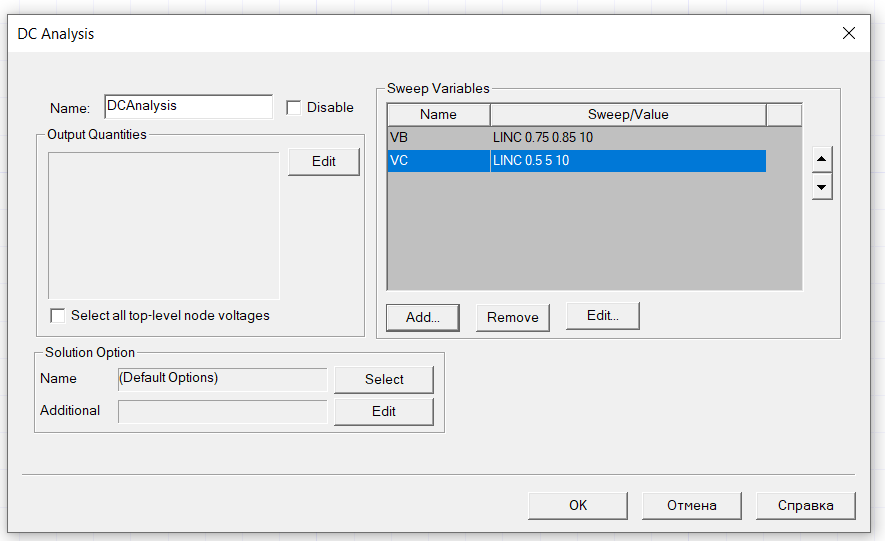
\includegraphics[width=0.7\textwidth]{10.PNG}
	\caption{Настроенные диапазоны изменения $V_B$ и $V_C$.}
	\label{fig:dc_setup_2}
\end{figure}

После запуска анализа на график выводится зависимость постоянного тока коллектора (значение измеряемое амперметром, например \verb|Ipositive(Ic)|) от напряжения коллектор-эмиттер $V_C$ при различных фиксированных значениях напряжения базы $V_B$. Полученное семейство выходных вольтамперных характеристик позволяет определить положение рабочей точки и является основой для последующего расчета максимальной выходной мощности каскада.

\begin{figure}[H]
	\centering
	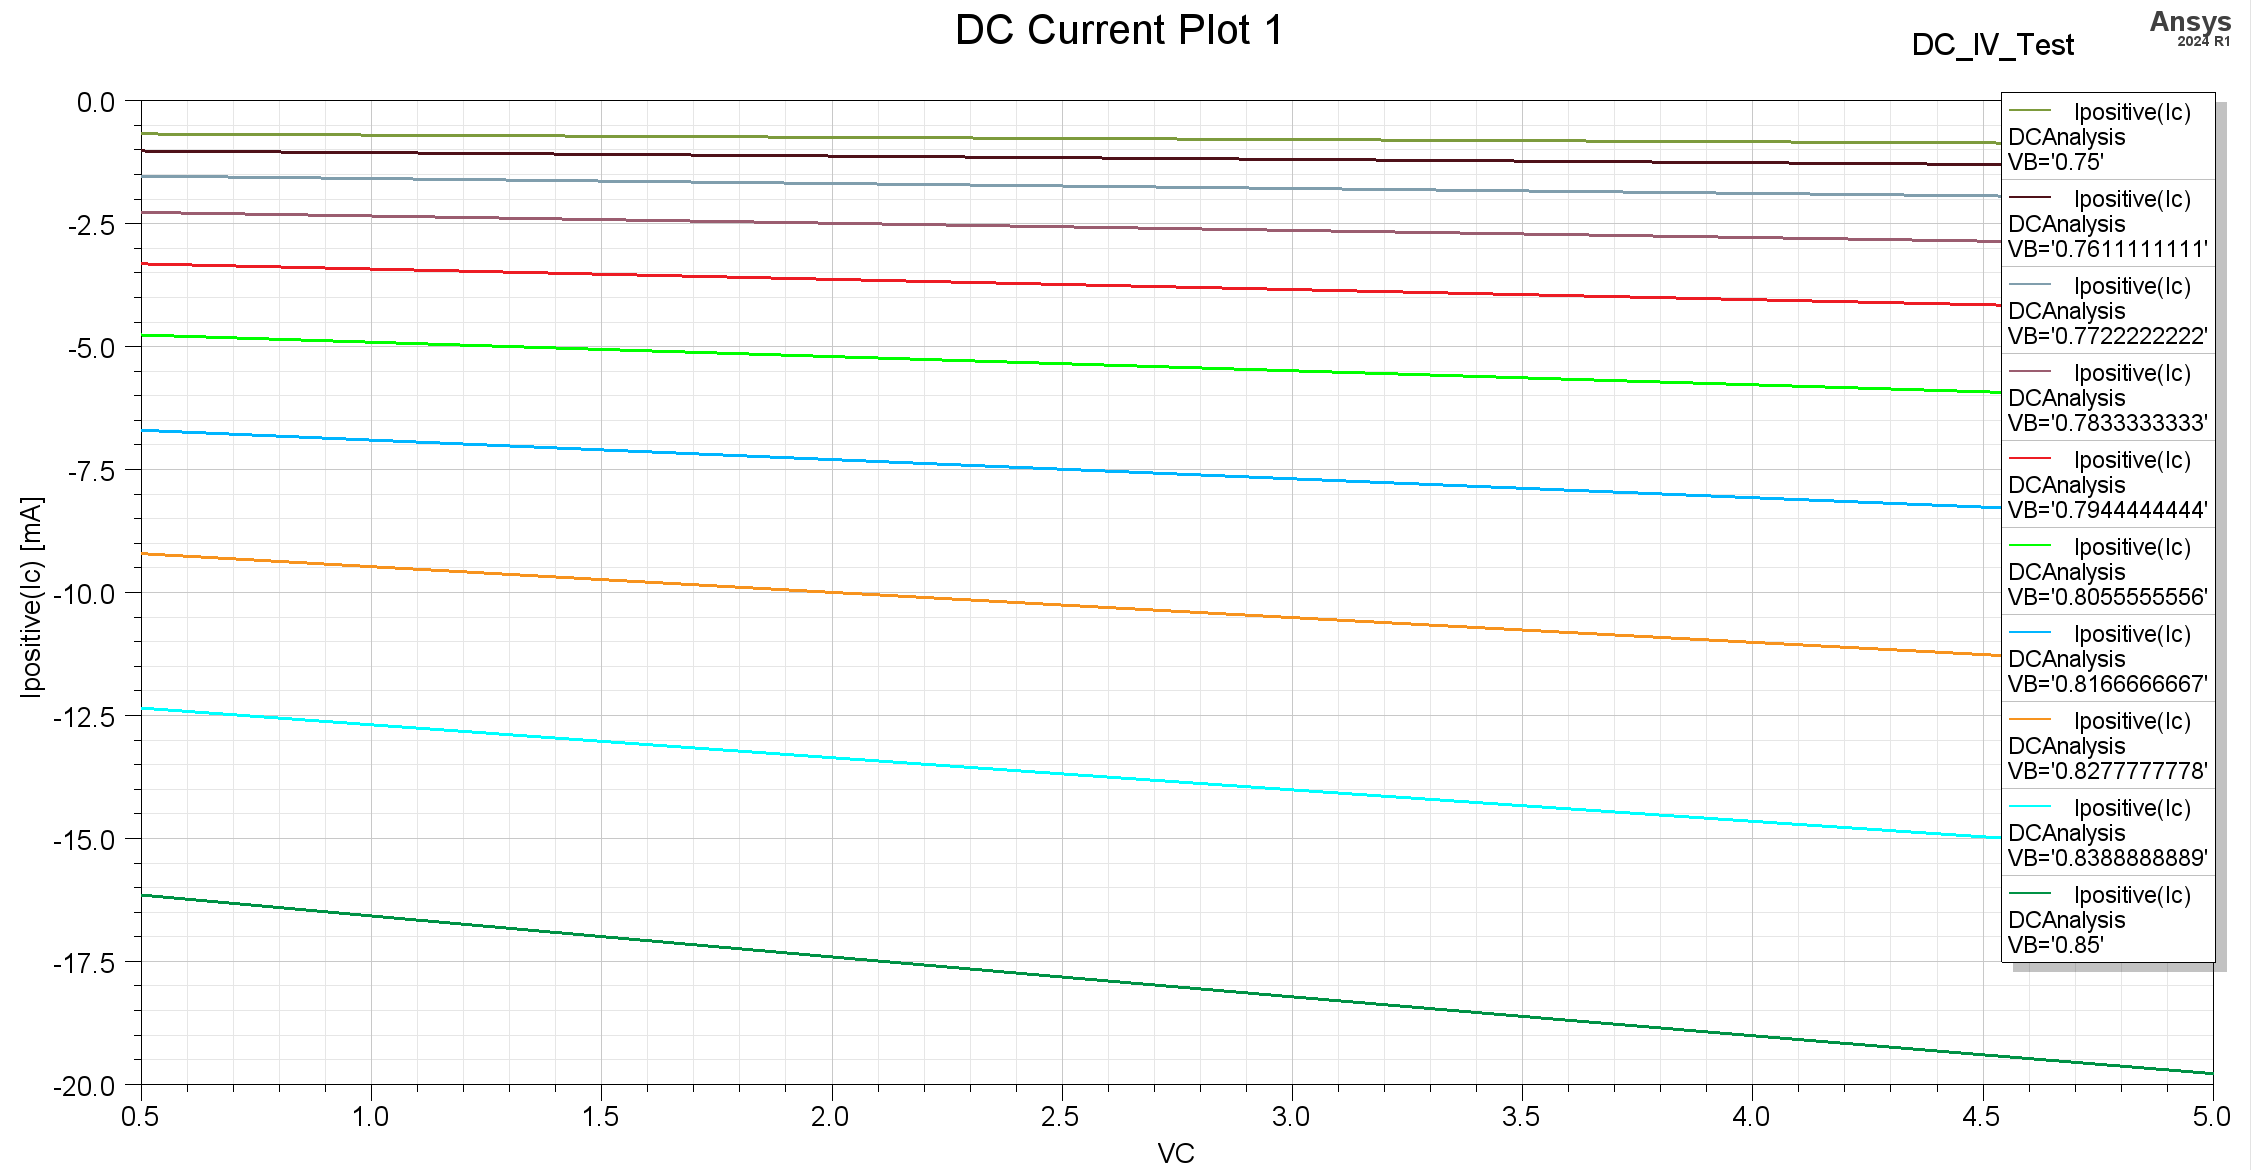
\includegraphics[width=0.9\textwidth]{11.PNG}
	\caption{Семейство выходных вольтамперных характеристик $I_c = f(V_C)$ транзистора NE68133.}
	\label{fig:dc_iv_curves}
\end{figure}